\chapter{Moving spiral wave chimeras (Physical Review E, 104(2), L022203)}

So far, this investigation has focused on drifting one-dimensional localized states in a non-local optical system. 
In these two cases, the motion itself was to be expected since a reflection
symmetry-breaking term was present. Nevertheless, such a term is not always
necessary to set localized states in motion. Indeed, this chapter exposes that motion can arise spontaneously
in an isotropic system of coupled phase oscillators.

In section~\ref{sec:phase_oscillators}, the importance
and universality of phase oscillators was emphasized, as they offer a comprehensive
description of self-sustained oscillators while neglecting the amplitude 
dynamics. Such oscillators are ubiquitous, they can be found in
in flashing fireflies, lasers, neurons, and even pacemaker cells in the heart.
Although the dynamics of an individual oscillator is already a challenging problem, as evidenced
by the Nobel Prize awarded to Hodgkin and Huxley for their neuron model
\cite{hodgkin1952quantitative},
exploring the dynamics of a population of coupled phase oscillators
introduces even greater complexity and richness. A fundamental question that
arises in these interacting oscillators systems is whether they will synchronize, 
and if so, to what degree?

While numerous authors made tremendous advances on this topic, one of the
most notable is Kuramoto who provided a simple yet powerful model 
for describing coupled oscillators several decades ago \cite{kuramoto1975model}. Even today, the Kuramoto
model and its modifications remain a very active research field [citas].
Remarkably, when Kuramoto and Battogtokh extended the model considering non-local coupling instead
of the original global coupling, he observed an incongruous state
of partial synchrony where coherent (synchronized) and incoherent (desynchronized) domains coexisted \cite{kuramoto2002coexistence}.
It could be expected that coupling identical oscillators would only yield a completely coherent
state, yet they showed that the symmetry could be spontaneously broken and the system
would self-organize into two different and coexisting domains, what we now call a chimera state \cite{abrams2004chimera}.

Even more surprisingly, two-dimensional simulations of the Kuramoto-Battogtokh model
revealed a planar chimera state in the form of a spiral wave. This spiral wave chimera
presented an incoherent core at the tip of the spiral where oscillators were desynchronized
while the remaining oscillators located in the spiral arms were synchronized. Similar spiral
patterns had already been observed in reaction-diffusion systems except for one significant
difference, the phase singularity located in the tip of the spiral was now replaced by
an incoherent core. Since then, spiral chimeras have been repeatedly observed both numerically [citas] and experimentally [citas]
in a variety of systems. 

In this chapter, we investigate the dynamics of a bound state of two counter-rotating spiral wave chimeras
 in a two-dimensional array of coupled non-identical
phase oscillators. To eliminate the finite-size noise, the
continuum limit of infinitely many oscillators is studied in detail
by numerically simulating the
associated Ott-Antonsen equation. Although a symmetric and isotropic coupling function is considered,
the top-hat function, a spontaneous symmetry breaking arises which causes
the two-core spiral chimeras to develop a permanent motion. Consequently,
the formation of a crescent-shaped filamentary pattern is observed in the incoherent core
of the spirals, and is oriented towards the direction of motion.  Moreover, we identify 3 
different two-core spiral chimeras according to their motion, namely symmetric, asymmetric
and meandering spirals, and determine their stability region.

% Sacar we, occur, one would think, no but, so , also, 
% pasado y presente perfecto.

% 2d extension: spiral wave chimera. similar to spiral wave, experiments, relevance
 
% in this chapter
% importance of synchronization. 
% synchronization: Huygens (history), Kuramoto (predictions, see section xx).
% one could expect they synchronize but chimera state! kuramoto battogtokh,
% experiments, etc. introduce spiral wave chimera

% in this chapter...

% Coupled oscillators, synchronization. Very important in many contexts, brain, heart,
% power grid, etc.

% Unexpectedly, a different state was also found: the chimera state. explain
% They have been predicted and experimentally observed in a plethora of systems
% [refs]. 

% In the weak coupling limit, these populations of nonlinear oscillators can be accurately
% described by a simple yet powerful model: the Kuramoto model. 


% This second half will be devoted to the study of coupled phase oscillators. As
% stated previously, in section~\ref{sec:phase_oscillators}, the dynamics of
% a non-linear oscillator, in the limit of weak coupling, can be reduced
% to a single cyclic variable: the phase. Therefore, an adequate and general model
% for a population of coupled oscillators  

% [synchronization in the brain] \cite{erra2017neuralsynchronization}

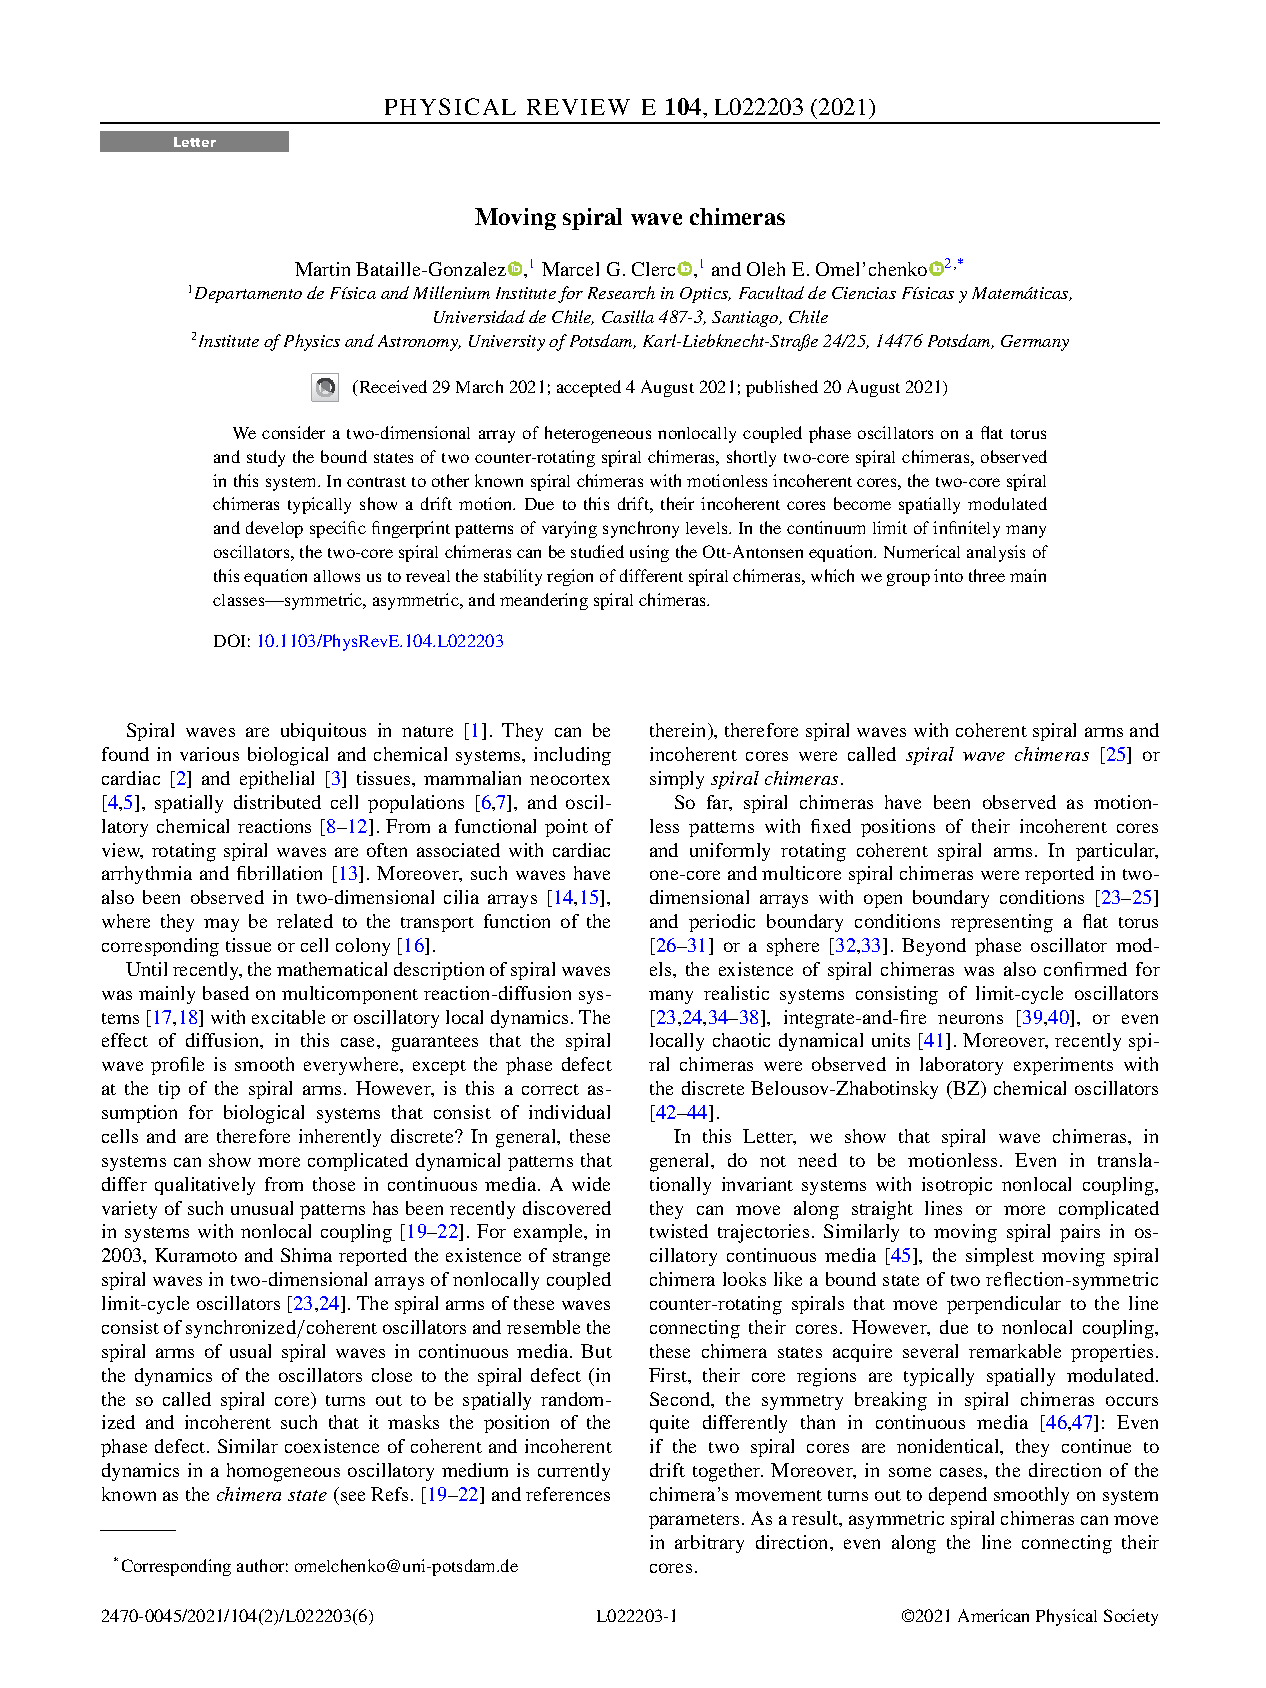
\includepdf[pages={-}]{chapters/movingspirals.pdf}

\section{Perspectives}
 

In this work, we have shown that even in a symmetric system, two-core
spiral chimeras move in three different ways. Furthermore, the stability region of symmetric, 
asymmetric and meandering spirals has been identified and presented in a phase diagram.
Nevertheless, a more in-depth numerical analysis is still needed to find not only
stable but also unstable states. This information will be fundamental to identifying
the various bifurcations that lead to the emergence of two-core spiral chimeras
from a homogeneous state, as well as the transition between symmetric and asymmetric
spirals. On the other hand, we have examined the effect of a top-hat coupling function
which has numerical advantages but may not be experimentally relevant. Therefore,
the extent to which these results extend to a more realistic coupling remains
to be determined.